\scanpage{25}

% Local layout keeps the long rules and detached marks beside the writing.
% Coordinates follow the supplied whole image; paper edges and punch holes are not ink drawings.
\figure{%
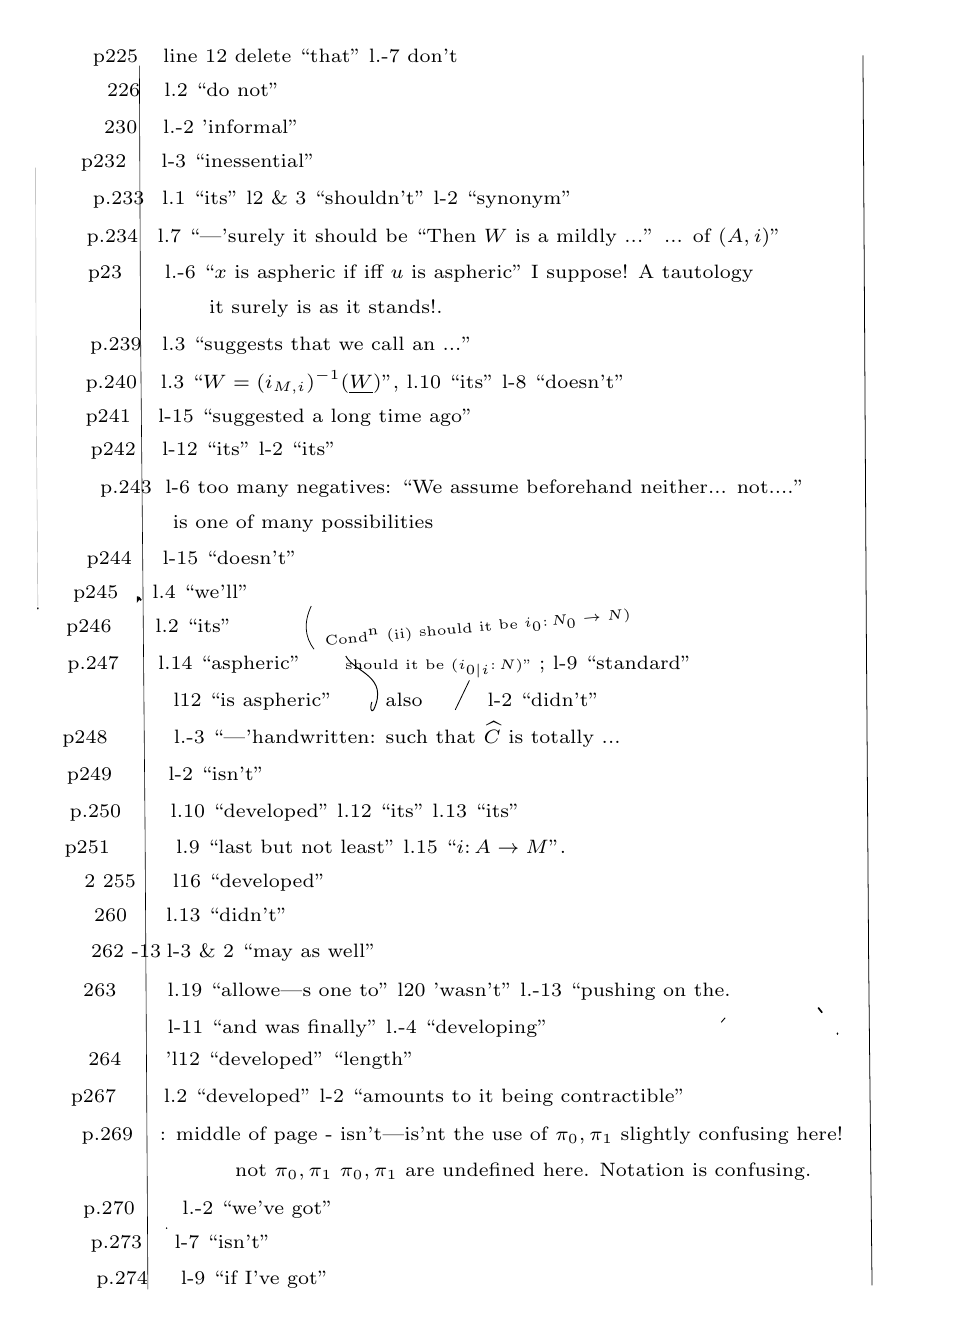
\begin{tikzpicture}[x=0.0072cm,y=-0.0072cm,every node/.style={anchor=base west,inner sep=0pt,font=\scriptsize}]
\path[use as bounding box] (35,45) rectangle (1640,2290);
% drawing-left-rule
\draw[line width=0.22pt] (232,112) -- (234,572) -- (238,1000) -- (242,1460) -- (247,2270);
% drawing-right-rule
\draw[line width=0.28pt] (1508,94) -- (1511,595) -- (1514,1120) -- (1518,1690) -- (1524,2263);
% drawing-far-left-trace: the purpose and medium of this faint trace are uncertain.
\draw[line width=0.15pt,opacity=0.35] (49,292) -- (50,685) -- (53,1065);
\fill (53,1069) ellipse [x radius=1.5,y radius=2.3];

% entry-01
\node at (149,106) {p225};
\node at (273,106) {line 12 delete ``that'' l.-7 don't};

% entry-02
\node at (174,167) {226};
\node at (275,167) {l.2 ``do not''};

% entry-03
\node at (169,231) {230};
\node at (273,231) {l.-2 'informal''};

% entry-04
\node at (128,292) {p232};
\node at (270,292) {l-3 ``inessential''};

% entry-05
\node at (149,356) {p.233};
\node at (271,356) {l.1 ``its'' l2 \& 3 ``shouldn't'' l-2 ``synonym''};

% entry-06
\node at (138,424) {p.234};
\node at (263,424) {l.7 \unsure{``|'}surely it should be ``Then $W$ is a mildly ...\deleted{\unsure{''}} ... of $(A,i)$''};

% entry-07
\node at (140,488) {\deleted{p23}};
\node at (276,488) {l.-6 ``$x$ is aspheric \deleted{\unsure{if}} iff $u$ is aspheric'' I suppose! A tautology};
\node at (354,549) {it surely is as it stands!.};

% entry-08
\node at (144,614) {p.239};
\node at (271,614) {l.3 ``suggests that we call an ...''};

% entry-09
\node at (136,681) {p.240};
\node at (269,681) {l.3 ``$W=(i_{M,i})^{-1}(\underline{W})$'', l.10 ``its'' l-8 ``doesn't''};

% entry-10
\node at (136,741) {p241};
\node at (264,741) {l-15 ``suggested a long time ago''};

% entry-11
\node at (145,799) {p242};
\node at (271,799) {l-12 ``its'' l-2 ``its''};

% entry-12
\node at (162,866) {p.243};
\node at (277,866) {l-6 too many negatives: ``We assume beforehand neither... not....''};
\node at (290,929) {is one of many possibilities};

% entry-13
\node at (138,992) {p244};
\node at (272,992) {l-15 ``doesn't''};

% entry-14
\node at (114,1052) {p245};
% drawing-p245-mark: the small angular mark is reproduced without assigning a punctuation function.
\draw[line width=0.6pt] (229,1048) -- (229,1055) -- (232,1051) -- (235,1055);
\node at (254,1052) {l.4 ``we'll''};

% entry-15
\node at (102,1111) {p246};
\node at (259,1111) {l.2 ``its''};

% entry-16: the written opening parenthesis of the raised insertion is drawn as the tall arc.
\node at (104,1176) {p.247};
\node at (264,1176) {\deleted{l.14 ``\unsure{aspheric}''}};
\draw[line width=0.28pt] (535,1065) .. controls (522,1093) and (523,1119) .. (540,1141);
\node[rotate=5,font=\tiny] at (559,1134) {\inserted{Cond\textsuperscript{n} (ii) should it be $i_0\colon N_0\to N$)}};
\node[font=\tiny] at (594,1176) {\deleted{should it be $(i_{\unsure{0|i}}\colon N)$\unsure{''}}};
\node at (936,1176) {; l-9 ``standard''};

% entry-17: also is physically beside the lower live correction, not before l-9.
\node at (291,1242) {l12 ``is aspheric''};
\node at (665,1242) {\inserted{also}};
\node at (845,1242) {l-2 ``didn't''};
% drawing-p247-curves: the first curve comes down from the cancelled proposal;
% the second stroke descends from the lower part of its opening parenthesis.
\draw[line width=0.35pt] (596,1153) .. controls (611,1182) and (673,1188) .. (645,1248) .. controls (641,1253) and (638,1246) .. (642,1234);
\draw[line width=0.3pt] (814,1196) -- (789,1248);

% entry-18
\node at (95,1307) {p248};
\node at (292,1307) {l.-3 \unsure{``|'}\uline{handwritten}: such that $\widehat C$ \uline{is} totally ...};

% entry-19
\node at (103,1372) {p249};
\node at (282,1372) {l-2 ``isn't''};

% entry-20
\node at (108,1437) {p.250};
\node at (286,1437) {l.10 ``developed'' l.12 ``its'' l.13 ``its''};

% entry-21
\node at (99,1501) {p251};
\node at (296,1501) {l.9 ``last but not least'' l.15 ``$i\colon A\to M$''.};

% entry-22
\node at (134,1562) {\deleted{\unsure{2}} 255};
\node at (290,1562) {l16 ``developed''};

% entry-23
\node at (151,1621) {260};
\node at (278,1621) {l.13 ``didn't''};

% entry-24
\node at (146,1684) {262 -\deleted{\unsure{13}}};
\node at (279,1684) {l-3 \& 2 ``may as well''};

% entry-25
\node at (132,1753) {263};
\node at (281,1753) {l.19 ``allow\unsure{e|s} one to'' l20 'wasn't'' l.-13 ``pushing on the.};
\node at (281,1819) {l-11 ``and was finally'' l.-4 ``developing''};
% drawing-p263-detached-marks
\draw[line width=0.32pt] (1258,1799) -- (1265,1791);
\draw[line width=0.6pt] (1429,1773) -- (1436,1782);
\fill (1463,1819) ellipse [x radius=1.6,y radius=2.2];

% entry-26
\node at (141,1875) {264};
\node at (277,1875) {'l12 ``developed'' ``length''};

% entry-27
\node at (110,1940) {p267};
\node at (274,1940) {l.2 ``developed'' l-2 ``amounts to \inserted{it} being contractible''};

% entry-28
\node at (129,2008) {p.269};
\node at (267,2008) {: middle of page - \deleted{\unsure{isn't|is'nt} the use of $\pi_0,\pi_1$ slightly confusing here!}};
\node at (400,2071) {\deleted{not $\pi_0,\pi_1$} $\pi_0,\pi_1$ are undefined \uline{here}. Notation is confusing.};

% entry-29
\node at (132,2138) {p.270};
\node at (307,2138) {l.-2 ``we've got''};

% entry-30
\node at (145,2197) {p.273};
% drawing-p273-point: this raised point is separate from the printed reference and the following l.
\fill (280,2162) ellipse [x radius=1.3,y radius=1.6];
\node at (293,2197) {l-7 ``isn't''};

% entry-31
\node at (155,2262) {p.274};
\node at (304,2262) {l-9 ``if I've got''};
\end{tikzpicture}%
}

% archive sheet number: 24
